\mysection{Méthodologie}

Compte tenu du problème et de ses contraintes, il faut préciser une méthodologie pour les aborder efficacement. La méthodologie proposée est composée de 5 étapes, comme indiqué dans le schéma de la figure \ref{fig:schema}. 

\begin{figure}[H]
	\begin{center}	
		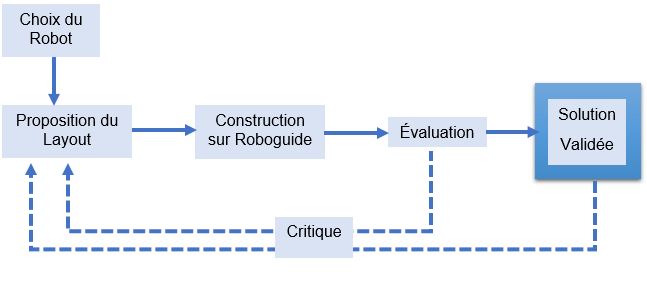
\includegraphics[width=\textwidth]{Methodologie/Representation.png}
		\caption{Représentation des étapes du projet}
		\label{fig:schema}
	\end{center}
\end{figure}


Au début, il faut \textbf{choisir un robot} parmi le catalogue Fanuc qui soit capable d’accomplir les tâches proposés, en termes de capacité de charge, vitesse et rayon d’action.
Ensuite, il faut \textbf{proposer le Layout}, c’est-à-dire, à partir des éléments fixes (cartons, palettes, robot) on choisit les autres éléments en quantité et dimensions adéquates, et on les arrange dans cellule.
Avec ces propositions, on passe au \textbf{logiciel Roboguide} pour les implémenter dans une cellule. Il faudra implémenter les objets, les positionner, programmer le mouvement du robot, animer les mouvements des objets et programmer le DCS. 
Une fois qu’on a une cellule fonctionnelle, on passe à \textbf{l’Évaluation}, étape dans laquelle les critères définis dans la section \ref{cadre} seront examinés, en mesurant  la surface, en déterminant le débit et en faisant des analyses de sécurité. \par \pagebreak Si la solution ne respecte pas même un des critères, elle est rejeté et on passe à la Critique, c’est-à-dire, on identifie les hypothèses explicites et implicites de la Proposition du Layout et essaye de les modifier, remplacer ou simplement rejeter.
Avec une solution validé en main il est possible de chercher une autre solution plus optimisée à travers du processus de Critique déjà présenté.
Lorsqu'on a plus qu'une solution on doit formuler un critère pour choisir la solution définitive. Le critère choisi par notre équipe était la surface de l’îlot: celui qui a la plus petite surface sera choisi.	
Avec ce schéma, l’équipe a fait trois cycles de développement, à partir desquels nous présentons la solution la plus optimisé. 